%%%%%%%%%%%%%%%%%%%%%%%%%%%%%%%%%%%%%%%%%
% Engineering Calculation Paper
% LaTeX Template
% Version 1.0 (20/1/13)
%
% This template has been downloaded from:
% http://www.LaTeXTemplates.com
%
% Original author:
% Dmitry Volynkin (dim_voly@yahoo.com.au)
%
% License:
% CC BY-NC-SA 3.0 (http://creativecommons.org/licenses/by-nc-sa/3.0/)
%
%%%%%%%%%%%%%%%%%%%%%%%%%%%%%%%%%%%%%%%%%

%----------------------------------------------------------------------------------------
%	PACKAGES AND OTHER DOCUMENT CONFIGURATIONS
%----------------------------------------------------------------------------------------

\documentclass[12pt,a4paper]{article} % Use A4 paper with a 12pt font size - different paper sizes will require manual recalculation of page margins and border positions
\usepackage[utf8]{inputenc}
\usepackage{marginnote} % Required for margin notes
\usepackage{wallpaper} % Required to set each page to have a background
\usepackage{lastpage} % Required to print the total number of pages
\usepackage[left=1.3cm,right=1.3cm,top=1.8cm,bottom=2.2cm,marginparwidth=3.4cm]{geometry} % Adjust page margins
\usepackage[fleqn]{amsmath} % Required for equation customization
\usepackage{amssymb} % Required to include mathematical symbols
\usepackage{xcolor} % Required to specify colors by name
\usepackage{xfrac}
\usepackage{fancyhdr} % Required to customize headers
\usepackage{booktabs}
\usepackage{xargs}
\usepackage{mathtools}
\usepackage{multirow}
\usepackage{graphicx}
\usepackage{lipsum}
\usepackage[linewidth=1pt]{mdframed}

\graphicspath{ {images/} }
\setlength{\headheight}{12mm} % Increase the size of the header to accommodate meta-information
\pagestyle{fancy}\fancyhf{} % Use the custom header specified below
\renewcommand{\headrulewidth}{0pt} % Remove the default horizontal rule under the header

\setlength{\parindent}{0cm} % Remove paragraph indentation
\newcommand{\tab}{\hspace*{2em}} % Defines a new command for some horizontal space

\newcommand\BackgroundStructure{ % Command to specify the background of each page
	\setlength{\unitlength}{1mm} % Set the unit length to millimeters

	\setlength\fboxsep{0mm} % Adjusts the distance between the frameboxes and the borderlines
	\setlength\fboxrule{0.25mm} % Increase the thickness of the border line
	%%\put(10, 15){\fcolorbox{black}{white!10}{\framebox(150,260){}}} % Main content box
	%%\put(150, 15){\fcolorbox{black}{gray!10}{\framebox(45,260){}}} % Margin box
%%	\put(10, 278){\fcolorbox{black}{white!10}{\framebox(192, 12){}}} % Header box
%% \put(137, 263){\includegraphics[height=23mm,keepaspectratio]{logo}} % Logo box - maximum height/width: 
}
\newcommand\const{\mathrm{const}}
\newcommand\solve[2]{\text{solve}\left\(#1\;\text{pour}\;#2\right\)}
%% \newcommand\vec\overrightarrow

\newcommand\textsup[1]{\ensuremath{^{\textrm{#1}}}}
\newcommand\textsub[1]{\ensuremath{_{\textrm{#1}}}}

%----------------------------------------------------------------------------------------
%	HEADER INFORMATION
%----------------------------------------------------------------------------------------

\fancyhead[L]{
	{\LARGE Formulaire de physique}
}
\fancyfoot[R]{
	{\small \thepage/\pageref{LastPage}}
}


%----------------------------------------------------------------------------------------

\begin{document}

\newcommand\formula[2]{#1 & = & #2}
\newcommand\nextcol{}
\newenvironmentx{twocols}[3][1=0.5, 2=0.4, 3=c]{
	\def\colonewidth{#1}
	\def\coltwowidth{#2}
	\def\mpagealign{#3}
	\renewcommand\nextcol{
		%%\vspace{0.4em}
		\end{minipage}
		\vrule\quad
		\begin{minipage}[\mpagealign]{\coltwowidth\textwidth}
		%%\vspace{0.4em}
	}
	\begin{minipage}[\mpagealign]{\colonewidth\textwidth}
	%%\vspace{0.4em}
}{
	%%\vspace{0.4em}
	\end{minipage}
}

\AddToShipoutPicture{\BackgroundStructure} % Set the background of each page to that specified above in the header information section

%----------------------------------------------------------------------------------------
%	DOCUMENT CONTENT
%----------------------------------------------------------------------------------------

\section{Mouvements}

\subsection*{Mouvement Rectiligne}
Mouvement d'un corps sur une trajéctoire réctiligne.
\subsubsection*{Uniforme (MRU)}
\begin{twocols}[0.5][0.5]
	$$
	\left\{
		\begin{array}{r c l}
			\formula{v}{\const} \\
			\formula{x}{x_0 + v \cdot t} \\
		\end{array}
	\right.
	$$
\nextcol
	\begin{tabular}{rcl}
		\formula{$v$}{Vitesse [$m/s$]} \\
		\formula{$x$}{Position [$m$]} \\
		\formula{$x_0$}{Position initiale [$m$]} \\
		\formula{$t$}{Temps [$s$]} \\
	\end{tabular}
\end{twocols}
\subsubsection*{Uniformément Accéléré (MRUA)}
\begin{twocols}
	$$
	\left\{
		\begin{array}{rcl}
			\formula{a}{\const} \\
			\formula{v(t)}{v_0 + a \cdot t} \\
			\formula{x(t)}{x_0 + v_0 \cdot t + \frac{a \cdot t^2}{2}} \\
		\end{array}
	\right.
	$$
\nextcol
	\begin{tabular}{rcl}
		\formula{$a$}{Accélération [$m/s^2$]} \\
		\formula{$v_0$}{Vitesse initiale [$m/s$]} \\
	\end{tabular}
\end{twocols}

\subsection*{Mouvement Circulaire}
Mouvement d'un corps autour d'un point de rotation (trajectoire circulaire).
\subsubsection*{Uniforme (MCU)}
\begin{twocols}[0.5][0.5]
	$$
	\left\{
		\begin{array}{rcl}
			\formula{\omega}{\const} \\
			\formula{\theta}{\omega \cdot t + \theta_0} \\
		\end{array}
	\right.
	$$
\nextcol
	\begin{tabular}{rcl}
		\formula{$\omega$}{Vitesse angulaire [$rad/s$]} \\
		\formula{$\theta$}{Angle [$rad$]} \\
		\formula{$\theta_0$}{Angle initial [$rad$]} \\
		\formula{$t$}{Temps [$s$]} \\
	\end{tabular}
\end{twocols}
\subsubsection*{Uniformément Accéléré (MCUA)}
\begin{twocols}
	$$
	\left\{
		\begin{array}{rcl}
			\formula{\alpha}{\const} \\
			\formula{\omega}{\omega_0 + \alpha \cdot t} \\
			\formula{\theta}{\theta_0 + \omega \cdot t + \frac{\alpha \cdot t^2}{2}} \\
		\end{array}
	\right.
	$$
\nextcol
	\begin{tabular}{rcl}
		\formula{$\alpha$}{Accélération angulaire [$rad/s^2$]} \\
		\formula{$\omega_0$}{Vitesse angulaire initiale [$rad/s$]} \\
	\end{tabular}
\end{twocols}

\newpage

\section{Balistique}

\begin{figure*}[h]
	\centering
	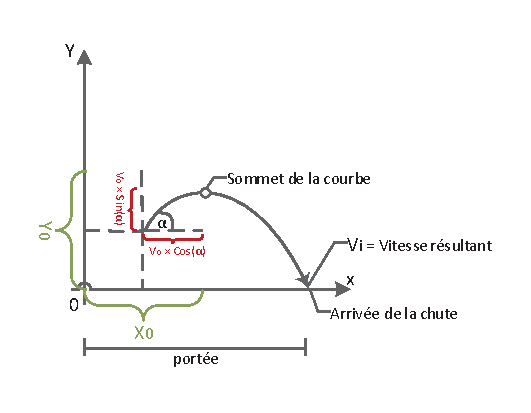
\includegraphics{Balistique}
\end{figure*}

\begin{twocols}[0.5][0.5]
	Acceleration
	\begin{equation*}
	\left\{
		\begin{array}{rcl}
			\formula{a_x}{0} \\
			\formula{a_y}{-g\;\text{OU}\;\const} \\
		\end{array}
	\right.
	\end{equation*}
	\par\vspace{1em}
	Vitesse
	\begin{equation*}
	\left\{
		\begin{array}{rcl}
			\formula{v_x(t)}{v_0 \cdot \cos{\alpha}} \\
			\formula{v_y(t)}{v_0 \cdot \sin{\alpha}-a_y \cdot t^2} \\
		\end{array}
	\right.
	\end{equation*}
	Position
	\begin{equation*}
	\left\{
		\begin{array}{rcl}
			\formula{x(t)}{x_0+v_0 \cdot \cos{\alpha} \cdot t} \\
			\formula{y(t)}{y_0+v_0 \cdot \cos{\alpha} \cdot t-\frac{a \cdot t^2}{2}} \\
		\end{array}
	\right.
	\end{equation*}

\nextcol
	
	Port\'ee
	\begin{equation*}
		\left\{
		\begin{array}{ll}
			p=\frac{v_0\,^2 \cdot \sin (2 \cdot \alpha)}{a} & \text{Si}\:y_0 = 0 \\
			p=\text{solve}\left(\left\{
					\begin{array}{rcl}
						y(t) & = & 0 \\
						x(t) & = & n \\
					\end{array}
			\right|
				\text{en} \: n
			\right)
			 & \text{Si}\:y_0 \neq 0
		\end{array}
		\right.
	\end{equation*}

	Alt. Maximale
	\begin{equation*}
		y_\text{max} = \frac{(v_0\cdot\sin{\alpha})^2}{2a} + y_0
	\end{equation*}

\end{twocols}

\vspace{1em}
\emph{Les unités sont identiques aux unités de la section MRUA}

\newpage

\section{Newton}
\subsection*{Lois de Newton}
\begin{mdframed}[leftmargin=2em, rightmargin=2em]
	\textbf{1\textsup{ere} loi de Newton} \\ \hspace{0.5em}
	%% Tout corps persévère dans l'état de repos ou de mouvement uniforme en ligne droite dans lequel il se trouve, à moins que quelque force n'agisse sur lui, et ne le contraigne à changer d'état.
	Tout corps dont la somme des forces est nulle est soit au repos, soit animé d'un mouvement rectiligne uniforme non accéléré.
\end{mdframed}
\par\hspace{1em}
\begin{mdframed}[leftmargin=2em, rightmargin=2em]
	\textbf{2\textsup{ème} loi de Newton} \\ \hspace{0.5em}
	%% L'altération du mouvement est proportionnelle à la force qui lui est imprimée ; et cette altération se fait en ligne droite dans la direction de la force.
	L'altération du mouvement est proportionnelle à la force qui lui est imprimée ; et cette altération se fait en ligne droite dans la direction de la force.	
	\begin{equation*}
		\overrightarrow{F} = m \cdot a
	\end{equation*}
	\begin{equation*}
		a = \frac{\sum \overrightarrow{F}}{\sum m}
	\end{equation*}
\end{mdframed}
\par\hspace{1em}
\begin{mdframed}[leftmargin=2em, rightmargin=2em]
	\textbf{3\textsup{ème} loi de Newton} \\ \hspace{0.5em}
	Pour chaque action, il existe une réaction égale et opposée.

	\begin{equation*}
		\sum\overrightarrow{F} = 0
	\end{equation*}
\end{mdframed}

\newpage

\subsubsection*{Lois dérivées}
Tirer un objet sur une pente \\
\begin{twocols}
	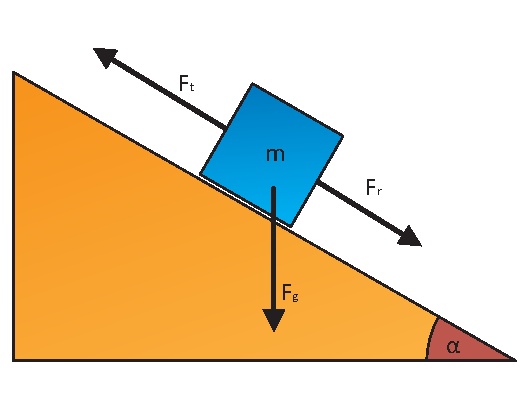
\includegraphics[height=4cm]{Newton-Pente}
\nextcol
	$$
		\left.\frac{\sum F_t - \sum R_r - F_g}{\sum m}\:\middle|
		\begin{array}{l}
			F_g = m \cdot g \cdot \sin\alpha \\
		\end{array}
		\right.
	$$
\end{twocols}
\par\vspace{1em}
Système de poulies \\
\begin{twocols}[0.5][0.5]
	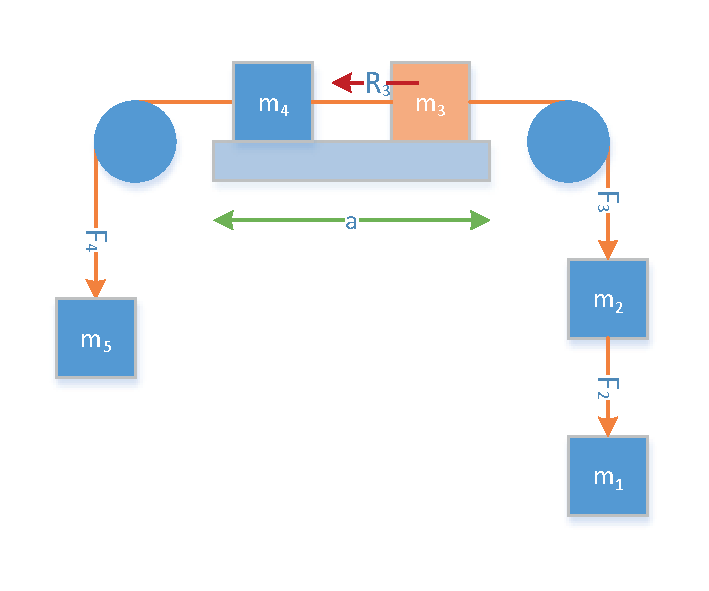
\includegraphics[width=1\textwidth]{Newton-Poulies}
\nextcol
	\begin{align*}
		a &= \frac{\sum F_n - \sum R_n}{\sum m_n} \\
		  &= \frac{g\cdot(m_1+m_2-m_5) - R_3}{m_1+m_2+m_3+m_4+m_5} \\
	\end{align*}
	\par\vspace{0.2em}
	Variables \\
	\begin{align*}
		F_n &= m_n \cdot g \\
		R_n &= \text{Résistance sur la masse $n$} \\
	\end{align*}
	\par\vspace{0.2em}
	{\small
	\textbf{notes} \\
	$F_n$ est nulle si l'objet n'est pas en suspension (ex $m_4$) \\
	Les masses qui ne sont pas en suspension et qui n'exercent pas de frottent sont tout de même comptées dans la somme des masses ($\sum m_n$)
	}

\end{twocols}

\newpage

\subsection*{Graviation Universelle}

	\begin{figure*}[h]
		\centering
		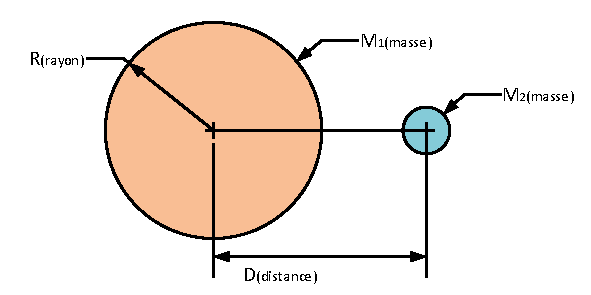
\includegraphics{Newton-Gravitation-1Planete}
	\end{figure*}

\begin{mdframed}[leftmargin=2em, rightmargin=2em]
	\textbf{Loi de la graviation universelle} \\ \hspace{0.5em}
	Deux corps quelconques s'attirent de manière proportionelle à leur masse et inversément proportionnelle au carré de leur distance. \\
	\par\hspace{0.5em}
	\begin{twocols}[0.3][0.3]
		$$\overrightarrow{F_G} = G\cdot\frac{m_1 \cdot m_2}{d^2}$$
		\nextcol
		\begin{tabular}{rcl}
			\formula{$F_G$}{Force de gravitation} \\
			$G$ & = & Gravitation universelle \\
				  & & $6.67 \times 10^-11$ \\
			\formula{$m_i$}{Masse} \\
			\formula{$d$}{Distance entre des corps} \\
		\end{tabular}
	\end{twocols}
\end{mdframed}
\par\hspace{1em}

\subsubsection*{Gravitation d'un corps}
\begin{figure*}[h]
	\centering
	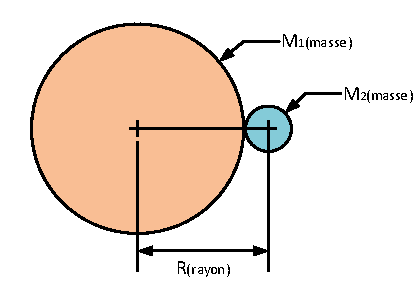
\includegraphics{Newton-Gravitation-Attraction}
\end{figure*}
Cette loi peut être dérivée pour lorsqu'un objet est suffisament proche d'un corps de masse plus importante que sa masse et taille new devienent insignifiants.

	$$\overrightarrow{F_G} = G\cdot\frac{m}{r^2}$$

\subsubsection*{Attraction entre deux champs de gravité}
\begin{figure*}[h]
	\centering
	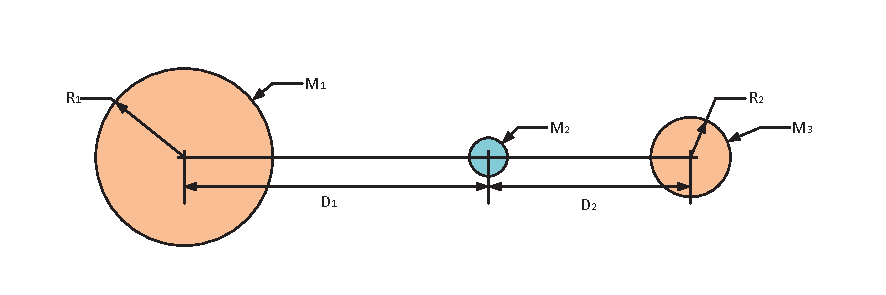
\includegraphics{Newton-Gravitation-2Planetes}
\end{figure*}
Une autre dérivation de cette loi peut s'appliquer lorsqu'un objet est soumis à deux champs de gravité distincts. Cette dérivation permet d'obtenir la direction et la vitesse avec laquel le corps au milieu se dirige.

	$$\overrightarrow{a} = G \cdot \left(\frac{m_1 \cdot m_2}{d_1\,^2} - \frac{m_3 \cdot m_2}{d_2\,^2}\right)$$

\subsubsection*{Équilibre d'attraction}
Lorsque l'objet se trouve à l'équilibre, l'accélération vaut 0. La formule peut donc être modifiée.

	$$\frac{m_1 \cdot m_2}{d_1\,^2} = \frac{m_3 \cdot m_2}{d_2\,^2}$$

\subsubsection*{Rapport des distances et des masses}
	$$\frac{d_1\,^2}{d_2\, ^2} = \frac{m_1}{m_3}$$

\newpage

\section{Statique}
La statique est l'étude des forces sur un système à l'équilibre, la somme de ses forces est donc nulle.

		$$\sum \vec{F} = 0$$

Les forces sont considérées comme des vecteurs est s'additionnenet donc comme tels.

\subsection*{Moment de Force}
Lorsqu'une force est appliquée sur un corps attaché à un axe de rotation, cette force produit un moment de force dont l'effet est propotionnel à la distance par rapport au centre de rotation et est mitigé par l'angle en fonction du corps.
\par\hspace{1em}
\begin{mdframed}[leftmargin=2em, rightmargin=2em]
	\begin{twocols}[0.5][0.5]
	$$
		\left\{
			\begin{array}{rcl}
			\formula{F_\perp}{F \cdot \sin \alpha} \\
			\formula{M}{F_\perp \cdot d} \\
			\end{array}
		\right.
	$$
	\nextcol
	\begin{tabular}{rl}
		$M$ & Moment de force \\
		$F_\perp$ & Force perpendiculaire \\
		$F$ & Force \\
		$\alpha$ & Angle de la force \\
	\end{tabular}
	\end{twocols}
\end{mdframed}

\newpage

\section{Transfert de chaleur}

\begin{twocols}
	
\begin{equation*}
	\begin{array}{r c l}
		\formula{\sum{Q}}{0} \\
		\formula{Q}{m\,c\,\Delta\theta} \\
		\formula{Q}{m\,C} \\
		\formula{\Delta\theta}{T_2 - T_2} \\
	\end{array}
\end{equation*}

\nextcol

	\begin{tabular}{rl}
		$Q$ & Energie [$J$] \\
		$\Delta\theta$ & Diff. de temperature [$\degC$]\\
		$m$ & Masse [$kg$] \\
		$c$ & Chaleur specifique [$\tfrac{J}{kg \cdot \degC}$] \\
		$C$ & Coefficient de transformation [$\tfrac{J}{kg}$]
	\end{tabular}


\end{twocols}

%----------------------------------------------------------------------------------------

\end{document}